\documentclass[11pt, reqno]{amsart}

\usepackage{amsmath}
\usepackage{amsfonts}
\usepackage{amsthm}

\usepackage{hyperref}

\usepackage[utf8]{inputenc}

\usepackage{tikz}
\usetikzlibrary{arrows}
\usetikzlibrary{backgrounds}

\usepackage{lipsum}

\usepackage{listings}

\usepackage{enumerate}
\usepackage{enumitem}

\usepackage{tabu}

\lstset{basicstyle=\ttfamily, mathescape=true}

\newcommand{\R}{\mathbb{R}}
\newcommand{\Q}{\mathbb{Q}}
\newcommand{\Z}{\mathbb{Z}}
\newcommand{\N}{\mathbb{N}}
\newcommand{\HH}{\mathcal{H}}
\newcommand{\BB}{\mathcal{B}}

\newtheorem{lemma}{Lemma}
\newtheorem{theorem}{Theorem}
\newtheorem{corollary}{Corollary}
\newtheorem{prop}{Proposition}

\newtheorem{definition}{Definition}

\newtheorem{conjecture}{Conjecture}

\newtheorem{remark}{Remark}

\DeclareMathOperator{\dig}{dig}
\DeclareMathOperator{\intr}{int}


\DeclareMathOperator{\len}{le}
\newcommand{\LE}{\mathbf{LE}}

\title[\textbf{Optimal bounds for $b$-ary measures}]{\textbf{On optimal bounds for comparing Dyadic (and $b$-ary) Net Measures with the Hausdorff Measure on $\R$}}


\author{Duarte Maia}
\address{Department of Mathematics, Instituto Superior Técnico}
\email{duarte.nascimento@tecnico.ulisboa.pt}


\author{Jorge Drumond Silva}
\address{Department of Mathematics, Instituto Superior Técnico}
\email{jsilva@math.ist.utl.pt}

\date{}


\begin{document}


\begin{abstract}
Hausdorff measure and Hausdorff dimension are topics of great importance in geometric measure theory. Besicovitch (1952) introduced the so-called `dyadic net measures' on $\R^n$, which serve as an estimate for the Hausdorff measure, allowing for easier calculation of Hausdorff dimension. In this paper, we generalize this notion to so-called `$b$-ary measures' and, for $n = 1$, investigate how well these measures estimate the Hausdorff measure, improving the classical bounds, and drawing connections to the theory of non-integer base digit expansions. We also make some attempt to understand how these $b$-ary measures are ordered as a function of $b$, and conclude with a proposition that shows that this is \emph{not} the order induced by the natural numbers, by constructing a set whose $b$-ary measure is a worse estimate of its Hausdorff measure when $b = 4$ than when $b = 5$.
\end{abstract}

\maketitle

\section{Introduction}

To aid in the study of Hausdorff dimension, Besicovitch (1952) introduced the notion of \emph{dyadic measure}, which is a modification of Hausdorff measure. The dyadic measure of a set usually differs from its Hausdorff measure, but the Hausdorff dimension of a set is always the same as its `dyadic dimension'. That is, the dimension of a set computed either with the Hausdorff measure or the dyadic measure is the same. The reason for this is an inequality of the form
\begin{equation}\label{hbineq1}
\text{Hausdorff measure} \leq \text{Dyadic measure} \leq C \times \text{Hausdorff measure},
\end{equation}
which ensures that both agree where they are either zero or infinity.

In this article, we intend to investigate inequality \eqref{hbineq1}.

We begin by generalizing the notion of dyadic measures in a natural way to what we have called $b$-ary measures, where $b$ represents a natural number greater than one. We denote the $s$-dimensional $b$-ary measure by $\BB_{bs}$, and show an inequality similar to \eqref{hbineq1}. In particular, we show that, for any set $E$,
\begin{equation}\label{hbineq2}
\HH_s(E) \leq \BB_{bs}(E) \leq (b+1) \HH_s(E).
\end{equation}

Later in this paper, we show a sharper version of \eqref{hbineq2}, by drawing a connection to the theory of $b$-ary digit expansions, which we will now explain. 

Define the function

\[ g_{bs} (t) = \inf_{x \geq t}\;\left(\parbox{18em}{the number obtained by interpreting the $b$-ary expansion of $x$ in base $b^s$}\right).\]
This function grows asymptotically like $t^s$. More concretely, it can be bound from below by $t^s$, and from above by $b t^s$.

The first of these bounds is sharp; the second is not. Indeed, we show that the problem of finding better bounds for \eqref{hbineq2} can be partially reduced to finding better bounds of the form $g_{bs}(t) \leq T t^s$. This leads us directly to our first main result:

\begin{theorem}
If $T$ is such that $g_{bs}(t) \leq T t^s$, the following inequality is true:

\[\BB_{bs}(E) \leq 2^{1-s} T \HH_s(E).\]

In particular,

\[\BB_{bs}(E) \leq 2^{1-s} \Theta \HH_s(E),\]
where $\Theta$ is the smallest $T$ satisfying the hypothesis.
\end{theorem}

In the other direction, in an attempt to investigate the sharpness of these estimates, we attempt to construct a set with as big a discrepancy between Hausdorff and $b$-ary measure as possible, again using the tools of $b$-ary digit expansions.

\begin{theorem}\label{clowerbound}
For each $b \in \Z_{\geq 2}$ there exists a dense collection of $s \in [0,1]$ for which there exists an $s$-set $E$ satisfying

\[\BB_{bs}(E) \geq 2^{1-s} \gamma^{-s} \HH_s(E)\]
where $\gamma$ is the smallest number whose $b$-ary digit expansion, when interpreted in base $b^s$, equals one.
\end{theorem}

Putting these two results together, we end up with the following bound for the optimal constant to replace $(b+1)$ by in \eqref{hbineq2}:

\begin{theorem}\label{cbounds}
Given $b$, $s$, let $C$ be the smallest real number such that the inequality

\[\BB_{bs}(E) \leq C \HH_s(E)\]
is true for all sets $E$. For $s$ in a dense subset of $[0,1]$, we have the bound

\[2^{1-s} \gamma^{-s} \leq C \leq 2^{1-s} \Theta,\]
where $\gamma$ and $\Theta$ are as defined above.
\end{theorem}

We conclude with the following application of this result.

Consider inequality \eqref{hbineq2}. \emph{A priori}, it seems to suggest that, as $b$ increases, the $b$-ary measures become increasingly worse estimates for the Hausdorff measure. This intuition is wrong, however, as evidenced by the following theorem, which states that, for $s = 1/2$, the 5-ary measure is actually a \emph{better} estimate than the 4-ary measure.

\begin{theorem}
Let $s = 1/2$. If $C$ is the optimal constant defined above, we have

\[C_{b = 5} < C_{b = 4}.\]
\end{theorem}

To this effect, we simply compute $\gamma_{b = 4}$ and $\Theta_{b = 5}$ to enough precision to allow us to show

\[\Theta_{b = 5} < \frac 1 {\sqrt{\gamma_{b = 4}}}\]
which, upon application of theorem \ref{cbounds}, shows the desired result.\footnote{It is also necessary to show that $1/2$ is in the dense set for which the inequality $C_{b=4} \geq 2^{1-2} \gamma^{-2}$ holds.}

\section{Net measures}

We begin by recalling the definition of Hausdorff measure and Hausdorff dimension.

Let $X$ be a metric space, with distance $d$. If $E \subseteq X$, we denote the diameter of $E$ by $\lvert E \rvert = \sup_{x, y \in E} d(x,y)$.

Given $E \subseteq X$, a \emph{$\delta$-covering} of $E$ is a countable collection of sets $\{U_n\}$ whose union contains $E$ and such that the diameter of any $U_n$ satisfies $0 < \lvert U_n \rvert \leq \delta$.

For every set $E \subseteq X$ and $\delta > 0$, define
\begin{equation}\label{hausdorffdeltadef}
\HH_s^\delta(E) = \inf \sum \lvert U_n \rvert^s
\end{equation}
where the infimum is taken over all $\delta$-coverings of $E$. When $s$ is fixed, given a covering $\{U_n\}$ of $E$, we refer to the quantity $\sum \lvert U_n \rvert^s$ as the covering's \emph{Hausdorff sum}.

Finally, define the Hausdorff measure of $E$ as
\begin{equation}\label{hausdorffdef}
\HH_s(E) = \lim_{\delta \to 0} \HH_s^\delta(E).
\end{equation}

Given a set $E$, the quantity $\HH_s(E)$ varies with $s$ in the following way: there exists an $s$ such that, for all $t > s$, $\HH_t(E) = 0$, and for all $t < s$, $\HH_t(E) = \infty$. This $s$ is what we refer to as the \emph{Hausdorff dimension of $E$.}

\smallskip

Hausdorff measure, and by extension Hausdorff dimension, is often very difficult to compute precisely since its definition requires one to look at all possible $\delta$-coverings. As such, there is interest in finding definitions that would allow simpler methods of computing, or at least estimating, these quantities.   

The notion of net measure arises from the idea of redefining the Hausdorff measure with a more manageable collection of sets to use for coverings. In the context of $\R^n$, Besicovitch (1952) used the so-called dyadic cubes, a construction we will generalize in a natural way to what we will call $b$-ary cubes. More extensive treatments can be found in \cite{falconer, rogers}.

We will be working solely on the real line. As a consequence, we will use the nomenclature `dyadic intervals' instead of cubes.

\begin{definition}
A subset of $\R$ is said to be a \emph{dyadic interval} if it is an interval of the form $\left[ k 2^j, (k+1) 2^j \right[$, for $k, j \in \Z$.

The dyadic measure is defined analogously to the Hausdorff measure, except that, instead of arbitrary coverings, we consider only $\delta$-coverings by dyadic intervals. It is denoted by $\BB_s(E) = \lim_{\delta \to 0} \BB_s^\delta(E)$.
\end{definition}

The usefulness of this definition lies in that, even though these measures do \emph{not} coincide in general with the Hausdorff measure, one can find bounds between them.

The following theorem is found in \cite{falconer, rogers} and is stated here without proof, though in the sequence of this article we will prove stronger results for the particular case of $n = 1$.

\begin{theorem}\label{badbound}
Consider the Hausdorff and dyadic measures defined on $\R^n$. For any set $E$, we have
\begin{equation}\label{badboundeq}
\HH_s(E) \leq \BB_s(E) \leq 3^n 2^{n^2} \HH_s(E).
\end{equation}
\end{theorem}

Theorem \ref{badbound} has the following consequence: if we define the ``dyadic dimension'' of a set analogously to how the Hausdorff dimension is defined, these two concepts would coincide. Indeed, the Hausdorff measure of a set is zero iff the dyadic measure is zero, and the same holds for when this measure is infinite.

Hence, if we are interested in the Hausdorff dimension of a set, we may begin by investigating its dyadic measure.

Notice, however, that the provided bound is not very sharp. Indeed, for $n = 1$ the constant given in inequality \eqref{badboundeq} amounts to 6, but we will see below that it can be significantly lowered without much effort. (And then lowered even more, with significantly more effort.)

Of course, this is of no consequence for dimensional considerations. However, the results that follow allow for much sharper bounds, and hopefully better understanding of how these two concepts relate.

\subsection{Hausdorff Coverings}

Notice that any monotone operation (that is, $f(E) \supseteq E$) that can be done on a set without increasing its diameter, or that can be parametrized as to increase it by arbitrarily small $\varepsilon$, can be assumed without loss of generality.

In the particular case of $\R$, we can assume that the sets we are using for coverings are intervals. Sometimes we will additionally assume that these intervals are closed, and sometimes we will instead assume them to be open. In any case, these hypotheses harm in no way the generality of the results obtained.

\section{Better elementary bounds}

The inequality $\HH_s \leq \BB_s$ is trivial. We will now proceed to establish a bound in the opposite direction.

\begin{prop}\label{easybound} For all $s \in \R^+_0$ the dyadic measure and Hausdorff measure obey the inequality
\begin{equation}\label{easyboundeq}
\BB_s \leq 3 \HH_s.
\end{equation}
\end{prop}

\begin{proof}
We will show that given any $\delta$-covering of $E$ we can construct a dyadic $\delta$-covering of $E$ such that its Hausdorff sum is at most three times bigger than the original's.

Given any $\delta$-covering $\{U_i\}$ of $E$, define $j_i$, for $i \in \N$, as the greatest integer such that $2^{j_i} < \lvert U_i \rvert$.

At most three intervals of the form $\left[ k 2^{j_i}, (k + 1) 2^{j_i} \right[$ intersect $U_i$, and their union covers $U_i$. Hence, we might consider the covering $\{I_i\}$ obtained from $\{U_i\}$ by replacing each $U_i$ by the intervals mentioned above. It is easy to verify this is also a $\delta$-covering of $E$, and it is trivial to check

\[\sum \lvert I_i \rvert^s \leq 3 \sum \lvert U_i \rvert^s.\]

Which concludes our proof.
\end{proof}

This bound, while twice as sharp as the one mentioned in equation \eqref{badboundeq}, can still be significantly improved. The proof, however, touches on what will be our main tool to try to control the bound. The idea is to find a way to replace any $\delta$-covering with a dyadic $\delta$-covering such that, if the first covering has Hausdorff sum $A$, the latter has Hausdorff sum at most $CA$, where $C$ is the upper bound on $\frac \BB \HH$ we desire to prove. Taking this a step further, we can focus merely on finding a way to, given an interval of length $\ell$, covering it by dyadic intervals of lengths $m_i$ such that $\sum m_i^s \leq C \ell^s$. One might have concerns about making sure that these dyadic intervals still form a $\delta$-covering, but that is not an issue, as we will see in the following lemma:

\begin{lemma}
Fix a dimension $s \in \R^+$ and suppose $C \in \R^+$ is such that, for any interval $I$ of length $\ell$, we can find a countable dyadic covering of $I$ by intervals $\{J_i\}$ of lengths $m_i$ such that
\[\sum m_i^s \leq C \ell^s.\]

Then $\BB_s \leq C \HH_s$.
\end{lemma}

\begin{proof}
This proof proceeds much like the proof of proposition \ref{easybound}, with one caveat.

Given some $E$, let $I_i$ be any $\delta$-covering of $E$ by intervals. For each $I_i$, let $\{J_{ij}\}_{j \in \N}$ be a collection of dyadic intervals such that  $\sum_j \lvert J_{ij} \rvert^s \leq C \lvert I_i \rvert^s$.

It is \emph{not} necessarily true that the collection $\{J_{ij}\}_{i,j \in \N}$ forms a $\delta$-covering, but it is easy to check that it forms at least a $C^{1/s} \delta$-covering, which shows $\BB^{C^{1/s} \delta}_s \leq C \HH^\delta_s$. Taking the limit as $\delta$ goes to zero, we get the desired result.
\end{proof}

\begin{remark} \label{dimnotzero}
We had to exclude from consideration the case $s = 0$ in this last proposition. Indeed, in all that follows \textbf{it should be assumed that $s \neq 0$}.
\end{remark}

\section{$b$-ary measures}\label{sectgenbmeasures}

In this section, we generalize the notion of dyadic measures in a natural way, by using powers of $b$ in place of powers of 2.

\begin{definition}
Define the $b$-ary intervals, where $b \in \N_{\geq 2}$, as those of the form
\[\left[k b^j, (k+1) b^j \right[, \;k, j \in \Z.\]

The definition for the $s$-dimensional $b$-ary measure, denoted $\BB_{bs}$, and the corresponding $\delta$-measures $\BB_{bs}^\delta$, should be evident by comparison to the definition of the dyadic one, using the $b$-ary intervals instead of the dyadic ones.
\end{definition}

The results of the last section can be translated into this slightly more general context without much added effort. We state the results without proof.

\begin{lemma}
Fix a dimension $s \in \R^+$, a base $b \in \N_{\geq 2}$, and suppose $C \in \R^+$ is such that, for any interval $I$ of length $\ell$, we can find a countable $b$-ary covering of $I$ by intervals $\{J_i\}$ of lengths $m_i$ such that
\[\sum m_i^s \leq C \ell^s.\]

Then $\BB_{bs} \leq C \HH_s$.

In particular, one can easily show that the premise is true for $C = b+1$, whence one gets the bound
\[\HH_s \leq \BB_{bs} \leq (b+1) \HH_s.\]
\end{lemma}

As mentioned in the introduction, it appears that, the bigger $b$ is (that is, the more pieces we divide our intervals in as $j$ decreases) the bigger the difference between $\HH_s$ and $\BB_{bs}$. This makes sense: as $b$ increases there is less we can discern because since there is a larger discrepancy between the size of one layer and the next we lose the ability to gauge more precisely the intermediate sizes.

This intuition proves to be partially correct. Indeed, if $b < c$ are both powers of a common integer, it is easy to check that any $b$-ary interval is also a $c$-ary interval, which implies the inequality $\BB_{bs} \leq \BB_{cs}$. This argument, however, is not generalizable.

It would be nice to have a criterion to, given two numbers $c, b \in \N_{\geq 2}$, tell if it is the case that $\BB_{bs} \leq \BB_{cs}$. One might conjecture that the $b$-ary measures are, in a sense, monotone as a function of $b$, but this turns out not to be the case, we we show at the end of this article. In other words, the following statement is \textbf{false}: If $c \geq b$ then $\BB_{bs} \leq \BB_{cs}$.\label{falseconjecture}

\section{Minimal interval coverings}\label{sec5}

We focus now on the following problem: given a dimension $s$ and an interval $I$, find a $b$-ary covering of $I$ with as small a Hausdorff sum as possible. We assume without loss of generality that $I$ is of the form $\left[ a, b \right[$ with $a < b$. These intervals will be refered to as \emph{half-open}.

We want to determine the least  $C$ such that, for any interval $I$, the following inequality holds
$$\BB_{bs}^\infty(I) \leq C \lvert I \rvert^s.$$
 This can be written as
\begin{equation}\label{defc}
C = \sup \frac{\BB_{bs}^\infty(I)}{\lvert I \rvert^s},
\end{equation}
where the supremum is taken over the half-open nonempty intervals $I$ and the usage of $\delta = \infty$ is intended to imply that any $b$-ary covering is admissible.

Notice, now, that an interval is uniquely determined by its length and its position. We can then write \eqref{defc} as
\[C = \sup_\ell \sup_\text{$I$ of length $\ell$} \frac{\BB_{bs}^\infty(I)}{\ell^s},\]
which is the same as
\[C = \sup_\ell \frac{\sup_{\lvert I \rvert = \ell} \BB_{bs}^\infty(I)}{\ell^s}.\]

Hence, we investigate $\sup \BB_{bs}^\infty(I)$, where the supremum is taken over intervals of a fixed length $\ell$.

We will now further restrict the class of intervals over which this supremum is taken. To be more precise, we will show
\[\sup_{\lvert I \rvert = \ell} \BB_{bs}^\infty(I) = \sup_{\substack{\lvert I \rvert = \ell\\ 0 \in I}} \BB_{bs}^\infty(I),\]
that is, that we can add the restriction that our intervals contain 0. To this effect, given any interval $I$ we will construct an interval $I'$, which has the same length and contains the origin, and we will prove that $\BB_{bs}^\infty(I') \geq \BB_{bs}^\infty(I)$.

Before performing the rigorous construction, here is a rough sketch of the idea. If we translate an interval by a multiple of $b^j$, for a fixed integer $j$, then the only coverings that we might be messing up are those that use intervals of size $b^{j+1}$ and above. Therefore, in order to minimize the perturbation induced by translating $I$ onto the origin, we translate it by a multiple of $b^j$ for the biggest possible $j$.

The rest of the proof consists of showing that covers using intervals of size bigger than $b^j$ are not problematic. The idea behind that is that the translate contains the origin, which forbids any `quick covers by big intervals', as no $b$-ary interval covers points on both sides of the origin.

[Perhaps here would be a good place to add an illustration. To do: think of what drawing would represent this proof.]

\begin{lemma}
Let $I$ be a half-open interval. Then, there exists a half-open interval $I'$ of the same length such that $0 \in I'$ and
\[\BB_{bs}^\infty(I') \geq \BB_{bs}^\infty(I).\]
\end{lemma}

\begin{proof}
Let $\ell = \lvert I \rvert$, and $j$ such that $b^j < \ell \leq b^{j+1}$.

\begin{enumerate}[label=\textbf{Case \arabic*:}]

\item \textbf{There exists $k$ such that $k b^{j+1} \in I$.}

In this case, let $I'$ be the interval given by translating $I$ by $-k b^{j+1}$. Then, it is clear that
\[\BB_{bs}^\infty(I') = \BB_{bs}^{b^{j+1}}(I'),\]
because any covering of $I'$ using an interval of size greater than $b^{j+1}$ can be `improved' by replacing it with a smaller interval. Furthermore, we have
\begin{equation}\label{transinvariance}
\BB_{bs}^{b^{j+1}}(I') = \BB_{bs}^{b^{j+1}}(I),
\end{equation}
because the translation done to turn $I$ into $I'$ preserves $b$-ary intervals of size $b^{j+1}$ or less.

These two, together with the fact that $\BB_{bs}^{b^{j+1}}(I) \geq \BB_{bs}^\infty(I)$, give us the desired inequality
\[\BB_{bs}^\infty(I') \geq \BB_{bs}^\infty(I).\]

\item \textbf{$I$ is contained in an interval of length $b^{j+1}$.}

In this case, 
\[\BB_{bs}^\infty(I) = \min(\BB_{bs}^{b^j}(I), b^{(j+1)s}).\]

There exists at least one point of the form $k b^j$ in $I$. Let $I'$ be given by translating $I$ by $-k b^j$. We proceed to compare $\BB_{bs}^\infty(I')$ and $\BB_{bs}^\infty(I)$.

\begin{enumerate}[label=\textbf{Subcase \roman*)}]

\item ($\BB_{bs}^\infty(I) = \BB_{bs}^{b^j}(I)$) By the same argument used to deduce equation \eqref{transinvariance}, we conclude
\[\BB_{bs}^\infty(I) = \BB_{bs}^{b^j}(I) = \BB_{bs}^{b^j}(I').\]

Furthermore, note that $\BB_{bs}^{b^j}(I') = \BB_{bs}^{\infty}(I')$, as any cover of $I'$ using an interval of size greater than $b^j$ would have a Hausdorff sum of at least $b^{(j+1)s}$, which is greater than $\BB_{bs}^{b^j}(I')$. In conclusion,
\[\BB_{bs}^\infty(I) = \BB_{bs}^\infty(I').\]

\item ($\BB_{bs}^\infty(I) = b^{(j+1)s}$) Observe that either
\[\BB_{bs}^\infty(I') = \BB_{bs}^{b^j}(I') \text{, or } \BB_{bs}^\infty(I') < \BB_{bs}^{b^j}(I').\]

In the first case $\BB_{bs}^\infty(I') = \BB_{bs}^{b^j}(I) \geq \BB_{bs}^\infty(I)$, as desired.

In the second case we can assert that $\BB_{bs}^\infty(I') \geq b^{(j+1)s} = \BB_{bs}^\infty(I)$ since we need only consider coverings that contain at least one interval of length $b^{j+1}$ and so have Hausdorff sum  at least $b^{(j+1)s}$.
\end{enumerate}
\end{enumerate}
\end{proof}

With this construction done, we have now shown that our problem can be reduced to determining
\[\sup_{\substack{\text{$I$ half-open interval}\\ 0 \in I}} \frac{\BB_{bs}^\infty(I)}{\lvert I \rvert^s}.\]

A simple observation about the origin is that any $b$-ary interval is either to the right or to the left of the origin, but no interval touches both sides. Therefore, we can consider our covering of the left side to be independent of our covering of the right side, leading quickly to the conclusion that, if $I = \left[ a, b \right[$ with $a \leq 0 \leq b$, we have
\[\BB_{bs}^\delta(\left[a, b\right[) = \BB_{bs}^\delta(\left[a, 0\right[) + \BB_{bs}^\delta(\left[0, b\right[)\]
for any $\delta \in \left]0, \infty \right]$.

Another observation, which we will soon justify rigorously (see lemma \ref{sidedoesntmatter}), is that $\BB_{bs}^\delta(\left[-\lvert a\rvert, 0\right[) = \BB_{bs}^\delta(\left[0, \lvert a\rvert\right[)$. This has the following consequence: if we define for $t \geq 0$ the function $g_{bs}(t) := \BB_{bs}^\infty(\left[0, t \right[)$, our problem becomes one of optimization. Indeed, our goal becomes to solve the optimization problem given by
\[ \sup_{\substack{\ell,r \in \R^+_0\\\ell+r \neq 0}} \frac{g_{bs}(\ell) + g_{bs}(r)}{(\ell + r)^s}, \]
and so we turn to studying the function $g_{bs}$, (we will often suppress the subscript when it is obvious from context and not particularly relevant) which has a connection to the theory of $b$-ary expansions of real numbers. Before proceeding, we finish this section by proving the property mentioned above:

\begin{lemma} \label{sidedoesntmatter}
For any base $b$, any dimension $s > 0$, and any $a \geq 0$, we have
\[\BB_{bs}^\delta(\left[-a, 0\right[) = \BB_{bs}^\delta(\left[0, a\right[).\]
\end{lemma}

\begin{proof}
Fix any $b$-ary $\delta$-covering of $\left[-a, 0\right[$. Denote it by $\{\left[x_i, y_i\right[\}$. Consider now the collection $\{\left[-y_i, -x_i\right[\}$. 

This collection almost forms a $b$-ary $\delta$-covering of $\left[0, a\right[$. Indeed, the only points that might not be covered are those of the form $-x_i$. This can, be remedied by augmenting our collection with intervals of the form $\left[ -x_i, -x_i + \varepsilon_i \right[$ with arbitrarily small $\varepsilon_i$, and so we reach the conclusion that there are coverings of $\left[0, a\right[$ with Hausdorff sum arbitrarily close to our original covering's. This proves that $\BB_{bs}^\delta(\left[-a, 0\right[) \geq \BB_{bs}^\delta(\left[0, a\right[)$. A similar argument will show the opposite inequality.
\end{proof}

\section{$b$-ary digit expansions (Introduction)}\label{sec6}

In the previous section we showed that a possible approach to the problem of tighter bounds on the $b$-ary measures would be to investigate the optimization problem given by

\[ \sup_{\substack{\ell,r \in \R^+_0\\\ell+r \neq 0}} \frac{g_{bs}(\ell) + g_{bs}(r)}{(\ell + r)^s}. \]

We now turn to the study of the function $g$.

\begin{remark}
In remark \ref{dimnotzero} we mentioned that we will be assuming $s \neq 0$. We will outline here another such assumption.

As $\R$ has Hausdorff dimension 1, for $s > 1$ both the $b$-ary and the Hausdorff measure of \emph{any} set in $\R$ will be zero. Then, the question of the relationship between these two is trivial and uninteresting. Therefore, \textbf{from now on, we always assume $s \leq 1$.}
\end{remark}

Let us now fix some $t > 0$, and investigate how one might go about calculating $g(t)$ given a dimension $s$ and a base $b$. (The case $t = 0$ is trivial, and thus not considered.) We recall the definition of $g$:

\[g_{bs}(t) := \BB_{bs}^\infty(\left[0, t \right[).\]

First, let $b^k$ be the least integer power of $b$ that is greater than or equal to $t$. Then, a possible covering of $\left[0, t \right[$ would be the interval $\left[0, b^k\right[$. Hence, $g(t) \leq b^{ks}$.

Now, observe that $b^{k-1} < t$, and so there is a maximal integer, which we will call $d_1$, such that $d_1 b^{k-1} \leq t$. This gives us another possible covering of our interval, given by
\[\left[0, b^{k-1} \right[, \left[b^{k-1}, 2 b^{k-1} \right[, \cdots, \left[d_1 b^{k-1}, (d_1 + 1) b^{k-1} \right[,\]
which yields another upper bound, $g(t) \leq (d_1 + 1) b^{k-1}$. Note that $d_1 < b$.

We can continue this process. If we let $d_2$ be maximal such that $d_1 b^{k-1} + d_2 b^{k-2} \leq t$ then the following sequence of intervals will cover $\left[0, t \right[$:
\begin{multline*}
\left[0, b^{k-1} \right[, \left[b^{k-1}, 2 b^{k-1} \right[, \cdots, \left[(d_1 - 1) b^{k-1}, d_1 b^{k-1} \right[ \\
\left[d_1 b^{k-1}, d_1 b^{k-1} + b^{k-1} \right[, , \cdots, \left[d_1 b^{k-1} + d_2 b^{k-2}, d_1 b^{k-1} + (d_2 + 1) b^{k-2} \right[,
\end{multline*}
giving us a new upper bound $d_1 b^{k-1} + (d_2 + 1) b^{k-2}$. Note, again, that $d_2 < b$.

We will make this process more rigorous shortly. Below is a diagram exemplifying it for $b = 3$ and $t = 0.86$.

%todo make slightly bigger?
\noindent\resizebox{\linewidth}{!}{
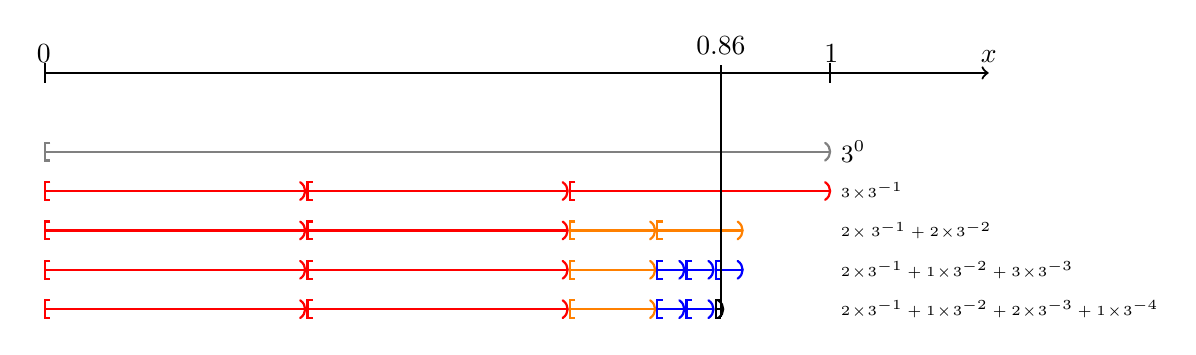
\begin{tikzpicture}
\draw[thick, {|-|}] (0,0) node[above]{0} -- (10,0) node[above]{1};
\draw[thick, {->}] (10,0) -- (12, 0) node[above]{$x$};

%The following was automatically generated with the help of the code at binary.py
\draw[thick, gray, {[-)}] (0, -1.0) -- (10, -1.0);
\draw (10, -1) node[right]{\small $3^0$};

\draw[thick, red, {[-)}] (0, -1.5) -- (3.333333333333333, -1.5);
\draw[thick, red, {[-)}] (3.333333333333333, -1.5) -- (6.666666666666666, -1.5);
\draw[thick, red, {[-)}] (6.666666666666666, -1.5) -- (10.0, -1.5);
\draw (10, -1.5) node[right]{\tiny $3\!\times\!3^{-1}$};

\draw[thick, red, {[-)}] (0, -2.0) -- (3.333333333333333, -2.0);
\draw[thick, red, {[-)}] (3.333333333333333, -2.0) -- (6.666666666666666, -2.0);
\draw[thick, orange, {[-)}] (6.666666666666666, -2.0) -- (7.777777777777777, -2.0);
\draw[thick, orange, {[-)}] (7.777777777777777, -2.0) -- (8.88888888888889, -2.0);
\draw (10, -2) node[right]{\tiny $2\!\times 3^{-1} + 2\!\times\!3^{-2}$};

\draw[thick, red, {[-)}] (0, -2.5) -- (3.333333333333333, -2.5);
\draw[thick, red, {[-)}] (3.333333333333333, -2.5) -- (6.666666666666666, -2.5);
\draw[thick, orange, {[-)}] (6.666666666666666, -2.5) -- (7.777777777777777, -2.5);
\draw[thick, blue, {[-)}] (7.777777777777777, -2.5) -- (8.148148148148147, -2.5);
\draw[thick, blue, {[-)}] (8.148148148148147, -2.5) -- (8.518518518518515, -2.5);
\draw[thick, blue, {[-)}] (8.518518518518515, -2.5) -- (8.888888888888886, -2.5);
\draw (10, -2.5) node[right]{\tiny $2\!\times\!3^{-1} + 1\!\times\!3^{-2} + 3\!\times\!3^{-3}$};

\draw[thick, red, {[-)}] (0, -3.0) -- (3.333333333333333, -3.0);
\draw[thick, red, {[-)}] (3.333333333333333, -3.0) -- (6.666666666666666, -3.0);
\draw[thick, orange, {[-)}] (6.666666666666666, -3.0) -- (7.777777777777777, -3.0);
\draw[thick, blue, {[-)}] (7.777777777777777, -3.0) -- (8.148148148148147, -3.0);
\draw[thick, blue, {[-)}] (8.148148148148147, -3.0) -- (8.518518518518515, -3.0);
\draw[thick, black, {[-)}] (8.518518518518515, -3.0) -- (8.641975308641975, -3.0);
\draw (10, -3) node[right]{\tiny $2\!\times\!3^{-1} + 1\!\times\!3^{-2} + 2\!\times\!3^{-3} + 1\!\times\!3^{-4}$};


\draw[thick] (8.6, 0.1) node[above]{0.86} -- (8.6, -3.1);
 
\end{tikzpicture}
}

\bigskip

Notice the structure of how we would find the $d_i$ in the previous argument: knowing $d_1, \cdots, d_{i-1}$, one would pick $d_i$ as the maximal one such that $\sum_{j = 1}^i d_j b^{k-j} \leq t$. This is, in fact, the exact same algorithm used to find the digits of $t$ in base $b$:

\fbox{
\parbox{\textwidth}{
Let $b^k$ be the least power of $b$ greater than $t$ for $t > 0$.

For $i = 1, 2, \dots$, define  $d_i$ as the maximal integer $d$ such that

\[ \left( \sum_{j = 1}^{i-1} d_j b^{k-j} \right) + d b^{k-i} \leq t.\]
}
}
\label{digalg}

Running this procedure for all natural $i$ in order, one will end with a sequence $\{d_i\}$ which corresponds to the digits of $t$ in base $b$. Indeed, in base $b$, $t$ would be represented as
\[t = d_1 d_2 \cdots d_k \, . \, d_{k+1} \ldots\]
or, in scientific notation,
\[t = b^k \times 0.d_1 d_2 d_3 \dots \]

All the $d_i$ are members of the set $\{ 0, \dots, b-1\}$, and furthermore we have
\[\sum_{i = 1}^\infty d_i b^{k-i} = t.\]

Finally, for any $N \geq 0$,
\[(\sum_{i=1}^N d_i b^{k-i}) + b^{k-N} \geq t.\]

As such, we may consider the collections of intervals given by

\begin{gather*}
\left\{\, \left[ x , x + b^{k-N} \right[ \;\middle|\; x = \left(\sum_{i=1}^N d_i b^{k-i}\right) + j b^{k-N}, 0 \leq j < d_N, 0 \leq N \leq M\,\right\}\\
\bigcup\\
\left\{\left[ \left(\sum_{i=1}^M d_i b^{k-i}\right) ,\left(\sum_{i=1}^M d_i b^{k-i}\right) + b^{k-M} \right[\right\},
\end{gather*}
for $M = 0, 1, 2, \dots$

To simplify the notation we make the following definitions:

\begin{definition}
Define $R_\delta(x)$ as the interval  $\left[x, x+\delta \right[$.

Let $\{d_i\}_{i \in \N}$ be a sequence of natural numbers. Define the collection of intervals denoted by
\[ b^k [d_0 d_1 d_2 \dots] \]
as follows:

First, define it inductively for finite sequences:

\begin{gather*}
b^k [] = \emptyset\\
b^k [d_0 \cdots d_n d_{n+1}] = b^k [d_0 \cdots d_n] \cup \left\{\, R_{b^{k-(n+1)}}(b^k \times d_0 . d_1 \cdots d_n j) \;\middle|\; 0 \leq j < d_{n+1} \,\right\}.
\end{gather*}

Then, for infinite sequences, simply take the increasing union
\[ b^k[d_0 d_1 \dots] = \bigcup_{i = 0}^\infty b^k[d_0 \cdots d_i].\]

\end{definition}

The proof of the following proposition is a time-consuming exercise, which is left to the reader.

\begin{prop}
Let $\{d_i\}_{i \in \N}$ be a sequence of natural numbers. Let $A = b^k [d_0 d_1 d_2 \dots]$. Then, $A$ satisfies the following properties:

\begin{itemize}
\item Every interval $I \in A$ is $b$-ary.

\item $\cup_{I \in A} I = \left[ 0, t \right[$, where $t = b^k \times d_0 . d_1 d_2 \dots$

\item Every two intervals in $A$ are disjoint.

\item The $s$-dimensional Hausdorff sum of $A$ is given by $b^{ks} \sum d_i b^{-is}$.
\end{itemize}

\end{prop}

\begin{remark}
Notice that the Hausdorff sum of $A$ can be easily written as a $b^s$-ary expansion. Namely, $(b^s)^k \times d_0 . d_1 d_ 2 \dots$

When writing numbers in scientific notation it is usually assumed that the base in which the expansion should be interpreted is the base of the mantissa, in this case, $b^s$. However, to save on parentheses, we will write abbreviate the previous expression to
\[b^{ks} \times d_0 . d_1 d_ 2 := (b^s)^k \times d_0 . d_1 d_ 2.\]

This is, in principle, an ambiguous expression, but we hope that it causes no confusion.
\end{remark}

Let $t$ have $b$-ary expansion $b^k \times d_0 . d_1 d_2 \dots$ Consider the coverings given by
\[ b^k [d_0 \cdots d_{n-1} (d_n + 1)] \]
as $n$ ranges over $\N$.

All of these cover $\left[0, t\right[$, and so we have

\[ g(t) \leq \inf \{\, b^{ks} \times d_0 . d_1 d_2 \cdots d_{n-1} (d_n + 1) \mid n \in \N\,\}.\]

This is, in fact, an equality.

\begin{prop} \label{ginfs}
Let $t$ have $b$-ary expansion $b^k \times d_0 . d_1 d_2 \dots$, with $d_0 = 0$.

Define $s_n = b^{ks} \times d_0 . d_1 d_2 \cdots d_{n-1} (d_n + 1)$ for $n \in \N$. Then,
\[ g(t) = \inf s_n.\]
\end{prop}

\begin{proof}
We already know $g(t) \leq \inf s_n$, so we only need to show the opposite inequality.

We will do this in two parts: first, we will show that the infimum required to compute $g(t)$ can be taken over coverings of the form $b^k [a_0 a_1 a_2 \dots]$. Then, we will show that any covering of this form has contribution that is at least $\inf s_n$.

Given an arbitrary $b$-ary covering $A = \{ I_i \}_{i \in \N}$ of $\left[ 0, t \right[$,
we may begin by supposing that there is no interval of size greater than $b^k$. Indeed, the only intervals greater than this size that are not immediately discardable are those of the form $\left[0, b^m \right[$ with $m > k$, but these can obviously be replaced by $\left[0, b^k \right[$ without any loss of generality. Furthermore, assume that all the intervals in $A$ are contained in $\left[0, b^k \right[$.

Define, inductively, the sequence $\{a_i\}_{i \in \N}$ as follows:

For all $n \in \N_0$, having defined $a_0 \cdots a_{n-1}$, let $a_n$ be the greatest natural such that $b^k [a_0 \cdots a_n] \subseteq \bigcup I_i$. Let $A'$ be the covering given by $b^k [a_0 a_1 \dots]$. We wish to show that this covering not only covers $\left[0, t \right[$, but also has Hausdorff sum less than or equal to that of $A$.

(review by duarte ends here)

First, we show that it covers the desired interval. We know $A'$ covers the interval from 0 up to $a = b^k \times a_0 . a_1 a_2 \dots$, so suppose for the sake of argument that $a < t = b^k \times d_0 . d_1 d_2 \dots$. It is easy to verify that if $a < t$ then there would exist $n$ such that, for $i < n$, we would have $a_i = d_i$, and $a_n < d_n$. But if this were the case, we would have a contradiction with our definition of $a_n$ by maximality, as it would mean that $b^k \times a_0 . a_1 \cdots a_{n-1} (a_n + 1) \leq t$ and so $b^k [a_0 \cdots a_{n-1} (a_n + 1)] \subseteq \bigcup I_i$.

So, we have established that $A'$ covers $\left[0, t\right[$. We will now show its Hausdorff sum does not exceed that of $A$.

First suppose, without loss of generality, that $\bigcup A$ is an interval of the form $\left[0,a\right[$. Then, it is easy to see that $b^k \times a_0 . a_1 a_2 \dots = a$ and therefore $\bigcup A = \bigcup A'$. With these hypotheses, as we will now show, any $I \in A$ is contained in some $J \in A'$.

Let $I \in A$ be of the form $R_{b^{k-n}}(i b^{k-n})$. Then, $a > (i+1) b^{k-n}$ and thus by the maximality of $a_n$, we have
\[ \sum_{i = 0}^n a_i b^{k-i} \geq (i+1) b^{k-n}. \]

Hence, the interval $I$ is contained in a union of $b$-ary intervals of $A'$ of at least its size, and since if two $b$-ary intervals intersect one of them must contain the other we conclude that $I$ is entirely contained in an interval in $A'$.

We can now finish the argument as follows: for each interval $J \in A'$ collect the intervals $I \in A$ contained in $J$. Note that, by what we have just seen, these cover $J$. We will show that each of these collections can be replaced by $J$ without increasing the Hausdorff sum, which allows us to conclude that the Hausdorff sum of $A'$ is at most that of $A$.

By elementary properties of the Lebesgue measure, we have
\[ \sum \lvert I \rvert \geq \lvert J \rvert,\]
from whence follows, by convexity and elementary calculus, that for $s \leq 1$ we have, as desired,
\[ \sum \lvert I \rvert^s \geq \lvert J \rvert^s.\]

This concludes the first part of the proof. We move on to the second part.

We have already concluded we need only consider coverings of the form $b^k [a_0 a_1 a_2 \dots]$ and, in fact, we need only take into account those constructed as above; this will allow us to use certain maximality arguments. We will now show that we may further restrict our attention to those sequences of the form $d_0 d_1 \cdots d_{n-1} (d_n + 1)$.

Given any arbitrary sequence $\{a_n\}$ constructed as above, we necessarily have $b^k \times a_0 . a_1 a_2 \ldots \geq b^k \times d_0 . d_1 d_2 \dots$ Then, either these two sequences are the same, or there exists a first index  where they differ. In the latter case, let $n$ be this index. That is, $a_i = d_i$ for $i < n$, $a_n \neq d_n$. It is necessarily the case that $a_n > d_n$ because, if $a_n < d_n$, we would reach a contradiction with the maximality of $a_n$. In this case we can safely assume our covering is of the desired form: indeed, the covering given by the sequence $d_0 d_1 \cdots d_{n-1} (d_n + 1) 0 0 0 \dots$ also covers $\left[0, t \right[$, and has Hausdorff sum not greater than that of the covering given by $\{a_n\}$.
As for the former case, consider the sequence $s_n$ we defined as $b^k \times d_0 . d_1 d_2 \cdots d_{n-1} (d_n + 1)$. We remark that $\lim s_n = b^k \times d_0 . d_1 d_2 \dots$. This limit is, in fact, the Hausdorff sum of the covering in consideration (that is, $b^k [d_0 d_1 d_2 \dots]$) and elementary calculus shows that $\lim s_n \geq \inf s_n$, as desired.

We have now, shown that whatever the covering we choose, $\inf s_n$ will be less than or equal than the Hausdorff sum of our covering, and therefore we have finally shown the result
\[ g(t) = \inf s_n.\]

\iffalse
Now, to show we can assume all intervals to be disjoint: fix any point $a$ in $\cup I_i$. Define $J_a$ to be \emph{the biggest interval in $A$ containing $a$}. We propose, now, that the covering $A' = \{ J_a \}$ covers exactly the same points as $A$, while having a Hausdorff sum less than or equal to that of $A$, as well as having all its intervals be disjoint.

The first two properties are trivial, so we devote our attention only to the third one: suppose, for the sake of argument, that $J_a$ and $J_b$ are not disjoint. The structure of the $b$-ary intervals mandates that either $J_a \subseteq J_b$ or $J_b \subseteq J_a$; suppose the former for the sake of argument. Then, $a \in J_b$, which implies $J_a$ is of length greater than or equal to that of $J_b$ (by definition), and so, in fact, $J_a = J_b$.

This digression completed, we may go back to the problem at hand.
\fi
\end{proof}

This last proposition has a few consequences, one of which is the following: it gives us an algorithm to approximate, or even compute, the value of $g(t)$, facilitating its study.

\section{$b$-ary digit expansions (Formalization)}\label{sec7}

We will now use the preceding proposition to study the function $g$ from another angle. We will begin by taking a closer look at the notion of digit expansion (also known as $\beta$-expansion). [I don't know what else to write here, but there is a paper coauthored by Erdös that seems to be the start of the area here: \url{http://www.numdam.org/article/BSMF_1990__118_3_377_0.pdf}. See also \url{https://mathscinet.ams.org/mathscinet/search/publdoc.html?pg1=MR&s1=142719&loc=fromreflist}. The main difference seems to be that I allow digits greater than $\lfloor b \rfloor$.]

\begin{definition}
We define a \emph{digit expansion} as a \emph{bounded} function $d : \Z \to \N$ for which
there exists $k$ such that, for $i < k$, we have $d_i = 0$.

\end{definition}

Given a base $b \in \left]1, \infty \right[$, to any digit expansion we can assign a real number. Indeed, by definition, the following sum, which we define as the `interpretation of $d$ in base $b$', converges:

\[ \sum_{i = -\infty}^\infty d_i b^{-i}.\]

Recall that any positive real number has a $b$-ary digit expansion. This expansion is not always unique, but the so-called `greedy expansion', the one obtained by the algorithm outlined in page \pageref{digalg}, is. This also happens to be the lexicographically largest digit expansion whose interpretation in base $b$ is precisely the number we started with. In this expansion, all the digits are contained in the set $\N \cap \left[0, b \right[$. Of course, for natural $b$, this is the familiar set of digits $\{0, \cdots, b-1 \}$, and natural bases have the benefit of almost-uniqueness: any number is uniquely determined by, and determines uniquely, a decimal expansion, as long as we restrict ourselves to those with digits in the set $\{0, \cdots, b-1 \}$ and that don't end with an infinite sequence of $b-1$.

We will use the notation $\dig_b t$ to mean the greedy digit expansion of $t$ in base $b$. In the other direction, given a digit expansion $d$ we use $\intr_b d$ to mean the interpretation of $d$ in base $b$.

\begin{remark}
It should be noted that there is a slight imprecision when we write expressions like ``let $b^k \times d_0 . d_1 d_2 \dots$ be the $b$-ary expansion of $t$''. Indeed, what we are saying here is not that the sequence $d$ is the expansion of $t$, at least not in the sense as above. Rather, the actual expansion would be something defined as follows:

\[d'_i =
\begin{cases}
d_{i-k} & \text{for $i \geq k$}\\
0 & \text{for $i < k$}
\end{cases}
\]

Furthermore, we often use that same notation to refer to both extracting the digits from a number, as well as to interpret a sequence of digits. This should not cause any confusion, however, as the operation being done is usually clear from context.
\end{remark}

We now propose an alternate definition of the function $g$.

As always, suppose fixed a base $b$ and a dimension $s$. We begin by defining, for $t \geq 0$,
\[ i_{bs}(t) = \intr_{b^s} \dig_b t.\]

This function will appear regularly in the sequence.

Now, we claim the following:

\begin{theorem} \label{ginfi}
For all $t \geq 0$,

\[g_{bs}(t) = \inf_{x \geq t} i_{bs}(x).\]
\end{theorem}

\begin{proof}
Suppose $t$ has $b$-ary expansion $b^k \times d_0 . d_1 d_2 \dots$. Let $t_n = b^k \times d_0 . d_1 d_2 \cdots d_{n-1} (d_n + 1)$.

We have already established that $g(t)$ can be calculated as $\inf s_n$, where $s_n = b^{sk} \times d_0 . d_1 d_2 \cdots d_{n-1} (d_n + 1)$.

We would like to argue that $s_n = i(t_n)$. Indeed, this is true under the condition that $d_n \neq b-1$, by almost-uniqueness of the $b$-ary expansion.

Of course, we can restrict ourselves to those $n$ such that $d_n \neq b-1$. Indeed, if $n$ satisfies this condition, it is trivial to check that $s_{n-1} \leq s_n$.

As a consequence, we conclude
\[g(t) = \inf_{\{n \mid d_n \neq b-1\}} i(t_n).\]

This shows $LHS \geq RHS$, as for all $n$ we have $t_n \geq t$.

For the other inequality, we will show $i(x) \geq g(t)$ for all $x \geq t$.

Consider the following three cases:


\begin{enumerate}[label=\textbf{Case \arabic*:}]

\item $x = t$. We already know that $i(t) = \lim s_n \geq g(t)$, so this case is done.

\item $x \geq b^{k+1}$. In this case $i(x) \geq b^{(k+1)s} > b^{ks} = s_0 \geq g(t)$.

\item $t < x < b^{k+1}$. Suppose $x$ has a $b$-ary expansion $b^k \times x_0 . x_1 x_2 \dots$ and let $n$ be the index such that $d_i = x_i$ for $i < n$ and $d_n \neq x_n$. Then, $d_n < x_n$, and therefore every digit of $t_n$ is less than or equal to its corresponding digit in $x$. Therefore, $i(x) \geq i(t_n) \geq g(t)$.
\end{enumerate}
\end{proof}

\section{$g$ as a function of $s$}

We now present an application of theorem \ref{ginfi} which will be useful in the sequence.

\begin{prop} \label{gfuncofs}
Fix arbitrary $t > 0$ and a base $b$. Define $h(s) = g_{bs}(t)$. Then, $h$ is a continuous function from $\left]0, 1 \right]$ to $\R$. Furthermore, for $t \in \left[0, 1 \right]$, $h$ is decreasing.
\end{prop}

\begin{proof}
We begin by showing $h(s)$ is decreasing.

Notice that for any $t \in \left[0, 1 \right]$ the function $t^s$ is a decreasing function. Therefore, for any $t \in \left[0, 1\right]$ we have $i_{bs}(t) = \sum d_i b^{-si} = \sum d_i (b^{-i})^s$, which is decreasing as a function of $s$.

Since $g_{bs}(t) = \inf_{x \geq t} i_{bs}(x)$, we can without loss of generality suppose $x \leq 1$, and then each of these terms is decreasing with $s$, the value of $g_{bs}(t)$ must also be decreasing with $s$, which completes the first part of the proof.

For the second half, we recall that $g$ can be defined as
\[g(t) = \inf s_n(t),\]
where, if we let $t$ have $b$-ary expansion $b^k \times d_0 . d_1 d_2 \dots$, $s_n(t)$ is defined as $b^{ks} \times d_0 . d_1 \cdots d_{n-1} (d_n + 1)$.

To show $g_{bs}(t)$ is a continuous function of $s$, it is not quite enough to show all $s_n(t)$ are continuous functions of $s$. It is, however, sufficient to show they are all Lipschitz with respect to a fixed constant $c$.

Indeed, notice that for any $n$ and $t$ the function $s_n(t)$ (of $s$) is a finite sum of terms of the form $\sum_i k_i b^{-is}$.  We can, then, take the derivative with respect to $s$, getting derivatives of the form $\sum - i k_i \log b \cdot b^{-is}$. Since all $k_i$ are at most, this sum is, in absolute value, less than $b \log b \sum i b^{-is}$, which converges to $\frac{b^{s+1} \log b}{(b^s + 1)^2}$ for $s > 0$.

Now the argument can be easily completed. Let $s > 0$. These derivatives are, in the interval $\left[s, 1 \right]$, all bounded by $c = \frac{b^{s+1} \log b}{(b^s + 1)^2}$, and so, in this interval, every $s_n(t)$ is $c$-Lipschitz as a function of $s$, and therefore so is $h$. This concludes the proof.
\end{proof}

\section{On notation}

Our main object of study is the `optimal constant' $C$ for the inequality $\BB_{bs} \leq C \HH_{bs}$. This constant depends on $b$ and $s$, and so, having fixed such a base and dimension, we call this optimal constant $C_{bs}$.

We have already shown that an upper bound to this constant is given by the solution to the optimization problem
\[ \sup_{\substack{\ell,r \in \R^+_0\\\ell+r \neq 0}} \frac{g_{bs}(\ell) + g_{bs}(r)}{(\ell + r)^s}.\]

We will call the solution to this optimization problem $K_{bs}$.

Subscripts will be omitted when $b$ and $s$ are fixed or implied from context.

\section{On calculating $K$} \label{calck}
%This section could go before introducing the bases, maybe?

In order to solve our optimization problem, we first make an observation about the function $g$: it is, in a sense, self-similar. Indeed, $g(b t) = b^s g(t)$. As such, it grows like $t^s$.

To be more rigorous, consider the interval $\left[ 1/b, 1 \right]$. The function that takes $t$ into $g(t)/t^s$ is continuous on this interval, and so, by Weierstrass's theorem, has a maximum and a minimum.

By convexity, $i(t) \geq t^s$, which, by the definition of $g$ using $i$, makes the inequality $g(t) \geq t^s$ evident. Equality is attained at, for example, $t = 1$.

The maximum turns out to be much harder to pinpoint, but in fact it is very closely related to $K$. To see why, let us give it a name, $\Theta_{bs}$, and let, for the moment, $\theta$ be a maximizer. It is clear that, while we took the maximum in $\left[ 1/b, 1 \right]$, the inequality $g(t) \leq \Theta t^s$ applies over all $\R^+_0$, and therefore

\[\frac{g_{bs}(\ell) + g_{bs}(r)}{(\ell + r)^s} \leq \frac{\Theta \ell^s + \Theta r^s}{(\ell+r)^s}.\]

The right hand side can be easily maximized with elementary calculus, giving us a maximum at $\ell = r$ of $2^{1-s} \Theta$, leading to the inequality

\[ 2^{1-s} \Theta \geq K.\]

The other inequality can be shown by noticing that, for $\ell = r = \theta$ the quantity to be maximized amounts to precisely $2^{1-s} \Theta$. This shows, then, that to calculate an upper bound of $C$ we can focus on trying to bound $g$ from above as closely as possible by a function of the form $\Theta t^s$. In other words, we are now interested in the optimization problem
\[ \max_{t \in \left[ 1/b, 1 \right]} \frac{g(t)}{t^s}.\]

Notice that the function being optimized is a quotient of two increasing functions. It is possible to approximate, to arbitrary precision, this class of functions. We present a naïve algorithm to this effect. [I don't know if there's any literature on this subject. Should I look into it?]
%note: i have a less naïve algorithm. should i present that?

\section{Optimization of increasing function quotients} \label{optimization}

Suppose that we have fixed an interval $I = \left[ a, b \right]$ and two continuous increasing functions $I \to \R^+$, call then $u$ and $v$. We focus on approximating the solution to the optimization problem

\[ \max_{t \in I} \frac{u(t)}{v(t)}.\]

Denote this maximum by $S$.

Consider a partition $P$ of I given by $a = t_0 < t_1 < \cdots < t_n = b$. For $i = 0, 1, \cdots, n-1$ define $M_i = \frac{u(t_{i+1})}{v(t_i)}$ and $m_i = \frac{u(t_i)}{v(t_{i+1})}$. Clearly, $M_i$ and $m_i$ are upper and lower bounds, respectively, of $u/v$ in the interval $\left[t_i, t_{i+1} \right]$. As such, if we let $M(P) = \max M_i$ and $m(P) = \max m_i$, we have the inequality
\[m(P) \leq S \leq M(P).\]

Of course, refining the partition will yield sharper bounds. Indeed, if $P_n$ is a sequence of partitions whose diameter converges to zero, $M(P_n) - m(P_n) \to 0$ by uniform continuity, and so each of these sequences will converge to $S$. This concludes this section on this kind of optimization problem.

\section{On the continuity of $K$}

In this section, we present the following result:

\begin{theorem}
As a function of $s \in \left]0, 1\right]$, the quantity $K_{bs}$ is continuous.
\end{theorem}

To this effect, we use the result of section \ref{calck} to reduce the matter to showing the following proposition:

\begin{prop}
As a function of $s \in \left]0, 1\right]$, the quantity $\Theta_{bs}$ is continuous.
\end{prop}

Recall that we defined $\Theta$ as

\[ \Theta_{bs} = \max_{t \in \left[ 1/b, 1 \right]} \frac{g(t)}{t^s}.\]

Hence, assuming $g_{bs}(t)$ is continuous as a function of $(s, t) \in \left]0, 1\right] \times \left[1/b, 1\right]$, which we will do shortly, we need only prove the following lemma:

\begin{lemma}
Let $X$ and $J$ be subsets of $\R$, and suppose $J$ is compact. Let $f$ be a continuous function $X \times J \to \R$.

We can define a function $u(x) : X \to \R$ defined as
\[ u(x) = \max_y f(x,y).\]

This function is continuous.
\end{lemma}

\begin{proof}
To show this lemma, consider a sequence $x_n \in X$ such that $x_n$ converges to some $x_0 \in X$. We will show $u(x_n)$ converges to $u(x_0)$.

Let $\varepsilon > 0$, and let $y_0$ be a maximizer of $f(x_0, y)$. There exists a neighbourhood, let's say $B_{\delta_1}(x_0) \times B_{\delta_2}(y_0)$ such that, for $(x,y)$ in this neighbourhood, $f(x,y)$ is within $\varepsilon$ of $f(x_0, y_0) = u(x_0)$, and so for $x \in B_{\delta_1}(x_0)$ we have $u(x) \geq u(x_0) - \varepsilon$.

On the other hand, consider the sequence $u(x_n)$. We can, without loss of generality, pass to a converging subsequence with limit $L$. The preceding argument shows $L \geq u(x_0)$; we now show the reverse inequality.

Let $y_n$ be a sequence of maximizers, that is, suppose it satisfies $f(x_n, y_n) = u(x_n)$. Suppose, again without loss of generality, that $y_n$ converges, to a limit $y_L$.

Then $L = \lim f(x_n, y_n) = f(x_0, y_L)$ by continuity. But, furthermore, $f(x_0, y_L) \leq u(x_0)$, which finishes our argument.
\end{proof}

[I think the preceding proof is needlessly complicated. I'll look into it again later]

We conclude the section with the following proposition:

\begin{prop}
Let $f : \left]0, 1\right] \times \left[1/b, 1\right] \to \R$ be defined as

\[f(s, t) = g_{bs}(t).\]

Then, $f$ is continuous.
\end{prop}

\begin{proof}
Notice that, for fixed $s$, $f$ is a continuous increasing function of $t$. [I just realized. I don't prove this anywhere. It is obvious? I'm pretty certain it's true, but I probably should prove this somewhere.] Furthermore, by proposition \ref{gfuncofs}, it is also a continuous decreasing function of $s$ for fixed $t \in \left[1/b, 1 \right]$. Elementary arguments show that, under these hypotheses, $f$ is continuous. %maybe i should be a bit less lazy here, huh?
\end{proof}

\section{A lower bound for $C$}\label{seclowerbound}

In the previous sections, we have constructed an upper bound for $C$, namely $K = 2^{1-s} \Theta$, using the tools of $\beta$-expansions and the function $g$. In this section, we will find a lower bound using those same methods.

Note that $g$ is a continuous increasing function, surjective from $\R^+_0$ to $\R^+_0$. This means that, for any $y$, there is a least $x$ such that $g(x) = y$. In particular, this is true for $y = 1$, and so we define $\gamma_{bs}$ as the corresponding $x$. It is obvious that $\gamma_{bs} \in \left] 1/b, 1 \right]$.

This quantity is useful because of the following property: consider the interval $\left[0, \gamma \right[$. There are many ways to cover it using $b$-ary intervals, but for purposes of minimizing the $s$-dimensional Hausdorff sum an optimal covering is the single interval $\left[0, 1 \right[$. Of course, this holds up to scaling by powers of $b$. We will use this quantity $\gamma$ to construct a set with the purpose of maximizing the discrepancy between the Hausdorff and the $b$-ary measure, and therefore obtain a lower bound for $C$.

\textbf{In what follows, we assume $0 < s < 1$.}

Fix an arbitrary dimension $s \in \left]0, 1 \right[$ and base $b$. We will build inductively a decreasing sequence of sets $S_n$, whose intersection, which we will call $S$, is the set we are looking for. To do this, we will define a transformation that, given $S_n$, will give us $S_{n+1}$.

Given an interval of the form

\begin{equation}\label{gableinterval}
I = \left] c b^\eta \pm \gamma b^\eta \right[
\end{equation}

we define the \emph{G-split of $I$} as the minimal collection of $b$-ary intervals whose reunion is $I$. For the interval $I_0 = \left]-\gamma, \gamma\right[$, this collection is simply given by all intervals in $b^0 [ d_0 . d_1 d_2 \dots ]$, where $d_i$ are the digits of $\gamma$, and their `symmetric' with respect to the origin, in the sense that the symmetric of $\left[a,b\right[$ is $\left[-b,-a,\right[$. For intervals $I$ of the more general form we can define their G-split by translating and rescaling $I$ to become $I_0$, taking its G-split, and doing the inverse translation and rescaling.

Now, given a $b$-ary interval $I$, define its \emph{A-split} by simply splitting $I$ into $b^\alpha$ congruent $b$-ary intervals. We have not yet specified $\alpha$; it is a free parameter, its only restriction being that it must be a nonnegative integer ($\alpha \geq 0$).

Finally, having fixed a $b$-ary interval $I = R_{b^\eta}(a)$, we define its \emph{B-split} as the interval $]c \pm b^{\eta - \beta} \gamma[$, where $c = a + b^{\eta - 1}$. Again, $\beta$ is an unspecified parameter, a positive integer $(\beta > 0)$. Notice that this is an interval of the form \eqref{gableinterval}, and therefore, an interval to which we can do a G-split. Another important property of the B-split is that, for any $b$-ary interval $I$, \emph{the smallest $b$-ary interval covering the entire B-split of $I$ is $I$ itself.}

Our construction consists of starting with an interval of the form \eqref{gableinterval} and simply applying G-splits, A-splits and B-splits repeatedly. This will give us the decreasing sequence of sets we are looking for.

More concretely, let $S_0 = \left]-\gamma, \gamma\right[$, and define $S_{n+1}$ as \emph{the B-split of the A-split of the G-split of $S_n$}. This process will give us a decreasing sequence of sets that depends on four parameters: $\alpha$, $\beta$, $b$ and $s$. We wish to manipulate these parameters to maximize the difference between the Hausdorff and $b$-ary coverings of $S$. We begin by inspecting the Hausdorff measure.

Note that all of the $S_i$, taken as unions of intervals, are Hausdorff covers of $S$. Let $\sigma_i$ be the Hausdorff sum of $S_i$.

Clearly, $\sigma_0 = (2 \gamma)^s$. Furthermore, by the recursive definition of $S_n$, which is invariant under rescaling, $\sigma_n$ is a geometric sequence, whose ratio between successive terms is simply $\frac{\sigma_1}{(2 \gamma)^s}$.

The only way for the limit to be nontrivial is for this sequence to be the constant sequence equal to one, and so for $\sigma_1$ to be $(2 \gamma)^s$. Hence, let us calculate $\sigma_1$.

First, calculate the Hausdorff sum of the B-split of $\left[0, 1 \right[$. The B-split of this interval is $\left] \frac 1 b - \frac \gamma{b^\beta}, \frac 1 b + \frac \gamma{b^\beta} \right[$, with Hausdorff sum $(2 \gamma)^s b^{-s \beta}$. By rescaling, the B-split of an interval of length $\ell$ would have Hausdorff sum $(2 \gamma)^s b^{-s \beta} \ell^s$.

Now, notice that before doing a B-split we first do an A-split. This means that an interval of length $\ell$ is turned into $b^\alpha$ many intervals, of length $\ell b^{-\alpha}$. Hence, the B-split of the A-split of an interval of length $\ell$ has Hausdorff sum equal to $b^\alpha (2 \gamma)^s b^{-s (\alpha + \beta)} \ell^s$.

If we have a set of intervals with Hausdorff sum $H$ and take their A and B-split the resulting Hausdorff sum is given by
\begin{align*}
\sum_\ell (2 \gamma)^s \ell^s b^{\alpha - (\alpha + \beta) s} &=
(2 \gamma)^s b^{\alpha - (\alpha + \beta) s} \sum \ell^s\\
&= (2 \gamma)^s b^{\alpha - (\alpha + \beta) s} H.
\end{align*}

Finally, we look at the Hausdorff sum of the G-split of an interval. Again, we will look at the interval $I_0 = \left] -\gamma, \gamma \right[$ as what will be said holds for arbitrary intervals by rescaling.

Half of the G-split of $I_0$ is given by $b^0 [ d_0 d_1 d_2 \dots]$, whose Hausdorff sum is simply $b^{0s} \times d_0 . d_1 d_2 \dots$. Since $i(\gamma) = g(\gamma) = 1$, the Hausdorff sum of the G-split of $I_0$ is 2.

Composing the three transforms, the Hausdorff sum of $S_1$ is given by

\[\sigma_1 = (2 \gamma)^s b^{\alpha - (\alpha + \beta) s} \cdot 2.\]

We need this to be equal to $\sigma_0 = (2 \gamma)^s$, and so we solve the equations to find parameters that make this true. In particular, we solve the equation

\[ 2 b^{\alpha - (\alpha + \beta) s} = 1,\]
yielding the result

\[s = \frac{\alpha + \log_b 2}{\alpha + \beta}.\]

For this particular dimension, we have shown $S$ has Hausdorff measure \emph{at most} $(2 \gamma)^s$. We will now bound from below the $b$-ary measure.

First, a technical lemma:

\begin{lemma}
Let $S \subseteq \R$ be compact. Then, the $s$-dimensional $b$-ary measure of $S$ can be computed through finite $b$-ary coverings of $S$.
\end{lemma}

\begin{proof}
Clearly, any finite $b$-ary covering is a $b$-ary covering. We need only show that any $b$-ary covering can be arbitrarily approximated by finite ones.

To this effect, fix a covering $\{ I_i \}_{i \in \N}$, where $I_i = \left[x_i, y_i \right[$. Augment it with the $b$-ary intervals $J_i = \left[x_i - \varepsilon_i, x_i \right[$, where $\varepsilon_i$ are such that their sum is at most some arbitrary $\varepsilon$. Then, the Hausdorff sum of the collection formed by all $I_i$ and $J_i$ is arbitrarily close to that of the initial covering.

Now, consider the collection of intervals $\{ \left]x_i - \varepsilon_i, y_i \right[ \}_{i \in \N}$. This is an open cover of $S$, and so, a finite subcovering, say $\{ \left]x_i - \varepsilon_i, y_i \right[ \}_{i \in \mathcal{I}}$, covers $S$. As such, we consider the collection of intervals of $I_i$ and $J_i$ with $i \in \mathcal{I}$; this collection is finite, covers $S$ and its Hausdorff sum is at most that of the original one plus an arbitrary $\varepsilon$, concluding our proof.
\end{proof}

This lemma is useful because $S$ is compact.

Indeed, it is trivial to see that the closure of the G-split of an interval $I$ is contained in $I$, which means the closure of $S_{n+1}$ is contained in $S_n$. This means that $S$ can be written as the intersection of all $\overline{S_n}$, all of which are compact, hence $S$ itself is compact. Therefore, we may bound the $b$-ary measure of $S$ from below by bounding the Hausdorff sum of \emph{finite} $b$-ary coverings of $S$.

We can further strengthen our assumptions. Notice that, for $n > 0$, $S_n$ contains no points of the form $k b^{-n}$. This implies that, given a finite $b$-ary covering of $S$, there exists $n$ such that our covering covers $S_n$, as we will now show.

Consider some finite $b$-ary covering of $S$. Let $n$ be a positive natural number such that all intervals of this covering have length greater than $b^{-n}$. Consider $S_n$ as a countable collection of intervals. Each of these intervals is either wholly contained in the covering we have fixed, or entirely outside it. Of course, if any of them were outside the covering, there would be at least one point of $S$ not being covered, which is a contradiction. Hence, $S_n$ is entirely covered.

Therefore, we now work with the following hypothesis: \textbf{Consider a \emph{finite} covering of some $S_n$}. If we can bound from below the Hausdorff sum of coverings of this kind, we have bound from below the $b$-ary measure of $S$, as desired.

We will now show by induction on $n$ that this covering has Hasudorff sum at least 2.

If $n = 0$ the result is a mere consequence of the definition of $\gamma$. We will now suppose that the result is true for some $n$, and show that it also holds for $n+1$.

Note that $S_{n+1}$ can be described as follows: consider all intervals $I = R_{b^\eta}(a)$ composing the A-split of the G-split of $S_0$ and replace each interval with an appropriately rescaled and translated copy of $S_n$, made to fit inside the B-split of $I$, which we will call $J = ]a \pm b^{\eta - \beta} \gamma[$. This allows us to use the induction hypothesis to assume, without loss of generality, that any $b$-ary cover of each of these copies of $S_n$ covers the entire interval $J$.

Any such cover is either a cover of $\left]-\gamma, \gamma \right[$ scaled down to the size of $J$, or contains an interval that covers $J$ entirely. Of course, in the latter case, because of a property of the B-split we mention above, we must actually cover $I$ entirely, yielding a Hausdorff sum of $b^{\eta s}$. In the former case, by rescaling, we have a Hausdorff sum of at least $2 b^{(\eta - \beta) s} = b^{\eta s} b^{\log_b 2 - \beta s}$. Since $\log_b 2 - \beta s = \alpha (s - 1) \leq 0$, at a minimum we have a Hausdorff sum of $b^{\eta s + \alpha (s - 1)}$.

What we have done refers to a single copy of $S_n$. Now, consider an interval $I = R_{b^\eta}(a)$ in the G-split of $S_0$. If we show that we can assume that $I$ is entirely covered, then we show that we can assume without loss of generality that we cover the entirety of $S_0$ and therefore that we have a Hausdorff sum of at least 2. Consider, then, an arbitrary $b$-ary covering of the copies of $S_n$ contained in the B-split of the A-split of $I$.

The A-split of $I$ consists of splitting $I$ into $b^\alpha$ identical intervals. We can assume, without loss of generality, that if we \emph{don't} cover the entirety of $I$ then each of these identical intervals is covered separately, with no interval in our covering containing two different intervals of the A-split of $I$. This means that we cover each of our copies of $S_n$ independently. Each of them, as we have shown, requires a Hausdorff sum of at least $b^{(\eta - \alpha)s + \alpha(s - 1)} = b^{\eta s - \alpha}$, and since there are $b^\alpha$ many of these, our $b$-ary cover has Hausdorff sum at least $b^{\eta s}$. This is the same as the Hausdorff sum of the trivial cover $\{I\}$, which means that we may assume $I$ is completely covered. This concludes our proof. \qed

[Need to review this proof]

To recap: our set $S$, built for any dimension of the form $s = \frac{\alpha + \log_b 2}{\alpha + \beta}$, satisfies
\begin{gather*}
\HH_s(S) \leq (2\gamma)^s\\
\BB_s(S) \geq 2
\end{gather*}
which shows that, for the dimensions $s$,
\[C \geq 2^{1-s} \gamma^{-s}.\]

Note that the set of dimensions $s$ for which we can conclude this inequality is rather small: countable, in fact, because the parameters $\alpha$ and $\beta$ vary over integers. However, it is easy to check that the set of possible dimensions forms a dense subset of $[0,1]$, and so we conclude

\begin{theorem}\label{boundtheorem}
Let $\Gamma_{bs} = \gamma_{bs}^{-s}$. Then,
\begin{equation} \label{partialineq}
2^{1-s} \Gamma_{bs} \leq C_{bs} \leq 2^{1-s} \Theta_{bs},
\end{equation}
where we have right inequality always holds and the left equality holds in a dense subset of $\left[0, 1 \right]$.
\end{theorem}

Since $\Gamma_{bs}$ is a continuous function of $s$ [Need to fact check this], if $C_{bs}$ is also continuous in $s$ then inequality \eqref{partialineq} holds for all $s \in [0,1]$. However, at time of writing, it is not known if this is true.

\section{Application}\label{secfinal}

We use the results from the preceding section to construct a set $S$ satisfying the property
\[ \BB_{5s}(S) < \BB_{4s}(S) \]
for some dimension $s$.

This is a rather striking result as it disproves the expected growth of the $b$-ary measures with $b$, mentioned in page \pageref{falseconjecture}.

In view of what we have already done, the set $S$ is not difficult to construct. Indeed, simply replicate the construction done above for $b = 4$, $\alpha = 0$  and $\beta = 1$, getting $s = 1/2$.

For this $S$, theorem \ref{boundtheorem} shows that $\BB_{4s}(S) \geq 2^{1-s} \Gamma_{4s} \HH_s(S)$. Furthermore, $\BB_{5s}(S) \leq K_{5s} \HH_s(S) = 2^{1-s} \Theta_{5s} \HH_s(S)$. We need now only show that  $\Theta_{5s} \leq \Gamma_{4s}$.

We begin by calculating $\gamma_{4s}$. We will show it is given by $4^0 \times 0.111\dots$, which equals $1/3$.

To show this, we begin by noticing that for any $t > 1/3$ we have $i(t) \geq 1$, which, together with the fact that $i(1/3) = 1$ shows that $g(1/3) = 1$.

Indeed, if $1/3 < t < 1$ (the case $t \geq 1$ is trivial), its ternary digits will agree with those of $1/2$ until some $n$-th digit, which will be a $2$ or a $3$. We then have
\begin{align*}
i(t) &\geq \frac 1 {4^s} + \frac 1 {4^{2s}} + \cdots + \frac 1 {4^{(n-1)s}} + \frac 2 {4^{ns}} \\
&= \frac 1 {2} + \frac 1 {2^2} + \cdots + \frac 1 {2^{n-1}} + \frac 2 {2^n} \\
&= 1.
\end{align*}

Now, notice that the numbers given by $t_n = \frac 1 2 - 4^{-n}$ converge to $1/2$, and $i(t_n)$ is always $< 1$, implying that for any $t < 1/3$ we have $g(t) < 1$.

We then conclude $\gamma_{4s} = 1/3$, whence $\Gamma_{4s} = \sqrt 3$.

We need now bound $\Theta_{5s}$ from above. To this effect, we use the strategy outlined in section \ref{optimization}

Consider the following partition of $\left[1/5, 1 \right]$:

\emph{Digit expansions should from now on be assumed to be in base 5}

\begin{center}
\begin{tabular}{| c | @{\qquad\qquad} | c | @{\qquad\qquad} | c | @{\qquad\qquad} | c |}
\hline
0.1 & 0.11 & 0.12 & 1 \\
\hline
\end{tabular}
\end{center}

Using the methods of section \ref{optimization}, and using proposition \ref{ginfs} to calculate $g(t)$, we construct the following table:

\begin{center}
\tabulinesep=1.2mm
\begin{tabu}{| c | | c | @{\qquad\qquad} | c | @{\qquad\qquad} | c | @{\qquad\qquad} | c |}
\hline
& 0.1 & 0.11 & 0.12 & 1 \\
\hline
$g(t)$ & & $\frac 1 {\sqrt{5}} + \frac 1 5$ & $\frac 1 {\sqrt{5}} + \frac 2 5$ & $1$ \\
$t^{-s}$ & $\sqrt 5$ & $\frac 5 {\sqrt 6}$ & $\frac 5 {\sqrt 7}$ & \\
\hline
\end{tabu}
\end{center}

And we then conclude that $\Theta_{5s}$ is bounded from above by

\[ \max \left\{ \left(\frac 1 {\sqrt{5}} + \frac 1 5\right) \sqrt 5, \left(\frac 1 {\sqrt{5}} + \frac 2 5\right) \frac 5 {\sqrt 6}, \frac 5 {\sqrt 7} \right\}.\]

Since all of these are strictly less than $\sqrt 3$, we conclude $\Theta_5s < \sqrt3 = \Gamma_4s$, and so
\[\BB_{5s}(S) \leq 2^{1-s} \Theta_{5s} \HH_s(S) < 2^{1-s} \Gamma_{4s} \HH_s(S) \leq \BB_{4s}(S),\]
as desired. \qed

\section{Acknowledgements}

The author would like to thank Jorge Drumond Silva for the initial suggestion to work in the topic of fractal geometry, and then the constant advice, orientation and fruitful discussions, throughout the 2018-2019 academic year, that culminated in this document. This work was developed within the framework of a scholarship of the Novos Talentos na Matemática program, from the Calouste Gulbenkian Foundation, to which the author is grateful. 


\begin{thebibliography}{1}
\bibitem{falconer}
Falconer, K. J. - \textit{The Geometry of Fractal Sets}, Cambridge University Press, Cambridge (1985).

\bibitem{rogers}
Rogers, C. A. - \textit{Hausdorff Measures}, 2nd ed., Cambridge University Press, Cambridge (1998).

\bibitem{brownian}
Shah, J. - \textit{Hausdorff Dimension and Its Applications}, available at http://www.math.uchicago.edu/~may/VIGRE/VIGRE2009/REUPapers/Shah.pdf

\bibitem{tao}
Tao, T. - ``From Rotating Needles to Stability of Waves: Emerging Connections between Combinatorics, Analysis, and PDE'', \textit{Notices of the AMS}, \textbf{48}, 294-303 (2001).

\end{thebibliography}


\end{document}
